\documentclass[journal=jpcbfk,manuscript=article]{achemso}

\usepackage{graphicx}
\usepackage{wrapfig}
\usepackage{subcaption}
\usepackage{amsmath} % or simply amstext
\usepackage{amssymb}
\usepackage{siunitx}
\usepackage{booktabs}
\usepackage[export]{adjustbox}
\newcommand{\angstrom}{\textup{\AA}}
\usepackage{cleveref}
\usepackage{booktabs}
\usepackage{gensymb}
\usepackage{float}
\usepackage{xr}
%\DeclareUnicodeCharacter{03C9}{$\omega$}
\externaldocument[S-]{Supporting_Information}

\SectionNumbersOn

\title{Statistical Inference of Transport Mechanisms and Long Time Scale Behavior from Time Series 
       of Solute Trajectories in Nanostructured Membranes}
\author{Benjamin J. Coscia}
\affiliation{Department of Chemical and Biological Engineering, University of Colorado Boulder, Boulder, CO 80309, USA}
\author{Christopher P. Calderon}
\affiliation{Department of Chemical and Biological Engineering, University of Colorado Boulder, Boulder, CO 80309, USA}
\author{Michael R. Shirts}
\email{michael.shirts@colorado.edu}
\affiliation{Department of Chemical and Biological Engineering, University of Colorado Boulder, Boulder, CO 80309, USA}

\begin{document}

  \graphicspath{{./figures/}}
  \maketitle
  
  \begin{abstract}

  Appropriate time series modeling of complex diffusion in soft matter systems on the
  microsecond time scale can provide a path towards inferring transport mechanisms and
  predicting bulk properties characteristic of much longer time scales. In this work 
  we apply the infinite hidden Markov model (IHMM) to solute center-of-mass trajectories
  generated from long molecular dynamics simulations in a cross-linked inverted hexagonal
  phase lyotropic liquid crystal (LLC) membrane in order to automatically detect a
  variety of solute dynamical states which can be further explained in terms of 
  solute-membrane interactions.

  We group the states identified by the IHMM into clusters based on multiple metrics
  aimed at distinguishing solute behavior based on their fluctuations, dwell times
  in each state and position within the inhomogeneous membrane structure. We analyze
  prevalent clusters in order to relate their parameters to physical interactions between 
  solutes and the membrane. 

  Along with parameters of individual states, the IHMM simultaneously infers a transition
  matrix which allows us to stochastically propagate solute behavior from all of the 
  independent trajectories onto much longer time scales while still preserving the 
  qualitative behavior characteristic of the MD trajectories. This affords a direct 
  connection to important macroscopic observables used to characterize performance like
  solute flux and selectivity. 
  
  Overall, this work provides an effective way to simultaneously identify transport 
  mechanisms in  nanoporous materials and project complex diffusive behavior on
  long time scales.  This enhancement to our understanding of the diverse range 
  of solute behavior allows us to hypothesize design changes 
  to LLC monomers aimed towards controlling the rates of solute passage, thus improving 
  the selective performance of LLC membranes. 
  

   
  \end{abstract}  
  
  
  \section{Introduction}
  
  % MRS: going to JPC, so emphasize the physical systems.
  There is a need for highly selective membranes in order to perform efficient 
  separations of the components of complex aqueous streams.
  \begin{itemize}
    \item Desalination and boric acid removal from seawater.
    \item Organic micropollutants
    \item Hydraulic fracturing flowback water
    \item Breathable chemical warfare agent barriers
    \item High purity chemicals
    \item While many researchers focus on membrane permeability, we may be 
    able to reduce costs of commercial nanofiltration and reverse osmosis with
    higher selectivity.~\cite{werber_materials_2016}
  \end{itemize}
  
  The ability to efficiently design novel membrane materials for selective separations
  would be greatly enhanced by easily interpretable methods for connecting microscopic
  fluctuations with macroscopic observables.
  %MRS: should explicitly point out that just calculating diffusion coefficients don't work for subdiffusive behavior, so
  %MRS need a different way to do it.
  %BJC2: added last two bullet points
  \begin{itemize}
  	\item If one could apply molecular dynamics (MD) simulations to explain important
  	experimental metrics such as solute flux and selectivity in terms of detailed 
  	chemically dependent solute motion, then we can more easily bridge the disconnect
  	between theory and application.
  	\item In many systems, it's possible to achieve this by calculating diffusion 
  	constants.\cite{}
  	\item Unfortunately, for systems which exhibit complex subdiffusive dynamics on the
  	time scales accessible to MD simulation, one cannot calculate reliable diffusion 
  	constants since solute mean square displacements (MSDs) are non-linear 
        %MRS2: added
        on timescales accessible to molecular simulation.
  	\item Therefore, we are in need of a more flexible approach for modeling solute 
  	dynamics which makes less assumptions about the solute's average behavior.
  	%BJC2: I'm moving these towards the end
%  	\item There are two main challenges associated with this goal.
%  	%since complex and
%  	%diverse diffusive motion on time scales accessible to molecular simulations prevents
%  	%us from easily relating chemically dependent solute motion to experimental time scales.
%  	\item First, we need a simple way to identify and parameterize the fluctuations
%  	characteristic to dominant solute-membrane interactions.
%  	\item Second, we need a way to propagate this behavior far beyond the time scales
%  	afforded by MD.
  \end{itemize}
  
  %MRS: point out that LLC's are examples where there are lots of hopping/jumping (cite previous papers) and
  %MRS: so we need different approaches.
  %BJC2: added last bullet point to lead in to following paragraph
  In this work, we are particularly interested in the design of lyotropic liquid crystal (LLC)
  monomers, a class of amphiphilic molecules whose ordered self-assembled phases can be 
  cross-linked into mechanically strong membranes capable of highly selective separations.
  \begin{itemize}
  	\item Inverted hexagonal, H\textsubscript{II}, phase LLC membranes are characterized
  	by hexagonally packed, uniform-sized and straight pores, an ideal geometry for high 
  	throughput transport.
	\item Their pores are lined with the LLC monomer functional groups which can
	potentially be designed to interact with solutes in a chemically-specific manner.
	\item It would be extremely useful to experimentalists if we could connect LLC monomer
	design with measurable quantities.
	\item This goal is complicated by the non-Brownian hopping and trapping behavior
	induced by the membrane's diverse topology and inhomogeneous structure.~\cite{coscia_understanding_2019,coscia_chemically_2019}
  \end{itemize}
  
  We have already progressed our understanding of LLC monomer design in our previous work
  by building stochastic time series models based on the chemical intuition gained
  from qualitative MD studies of solute transport in an H\textsubscript{II} phase LLC
  membrane.~\cite{coscia_chemically_2019,coscia_capturing_2020}
  \begin{itemize}
    \item We identified three classes of trapping behavior which result in short time scale
    subdiffusion.
    \item In our first approach to stochastically model this behavior, we treated the
    system's dynamics as a sequence of anti-correlated hops between power law distributed
    periods of entrapment, a framework called subordinated fractional Brownian or L\'evy
    motion.
    \item In a second approach, we treated solute motion as a Markov state model with 
    state-dependent dynamics, where we parameterized the state transition probabilities 
    between each of eight discrete states, defined by the observed trapping mechanism, 
    as well as the solute dynamics within each of these states. 
    \item We showed how one could use realizations of any stochastic model like these in
    order to predict macroscopic flux and selectivity. 
  \end{itemize}
  
  Although powerful and insightful, our previous work required considerable human effort
  in order to analyze the MD trajectories and to hypothesize stochastic models which
  matched the behavior of solutes.
  \begin{itemize}
    \item It would be significantly more useful and broadly applicable if we could 
    design an approach which automatically distinguishes and parameterizes varied solute 
    dynamics and leaves a facile way to generate an ensemble of stochastic trajectory
    realizations that can be used to predict macroscopic transport properties.
  \end{itemize}
  
  In this work we attempt to minimize human effort by applying the infinite hidden 
  Markov Model (IHMM)~\cite{beal_infinite_2002,calderon_inferring_2015}, a nonparameteric 
  Bayesian classification technique, in order to automatically detect and infer the 
  parameters of an unknown number of latent vector autoregressive (VAR) modes present 
  in solute center-of-mass time series trajectories. 
  \begin{itemize}
    %MRS: start with where it has been used before (to establish utility) a
    \item It's been used extensively for speaker diarization and has found some application
    in single particle trajectory analysis.
    %MRS: Then say it hasn't been used in this context (do we know of any, then cite, if none we have found, say so.)
    \item The IHMM has not been used much for MD trajectory analysis.

  \end{itemize}
  
  We aim to address two primary scientific 
  questions with this work. 
  First, we want
  to know if the IHMM algorithm can help researchers efficiently uncover underlying
  transport mechanisms which give rise to different solute dynamical behavior.
  Second, we want to predict macroscopic transport by using our model to generate 
  stochastic solute trajectories at much longer timescales than possible with MD simulations, 
  extending into timescale where diffusive behavior again occurs.
  
  We use the parameters of the states identified by the IHMM in order to infer 
  dominant solute-membrane interactions and transport mechanisms. We cluster similar 
  state parameters in order to reduce the state space and to understand which segments 
  of the solute trajectories exhibit similar behavior. We support our mechanistic 
  hypotheses via quantitative comparison to various physical membrane properties and
  solute-membrane interactions.
  
  Finally, we use the VAR parameters and state transition probability matrix in
  order to generate stochastic trajectory realizations with behavior similar to that
  exhibited by MD. 
  \begin{itemize}  
    \item One can project these realizations onto much longer timescales with 
    computational ease and use them to predict macroscopic properties.
  \end{itemize}
     
  \section{Methods}
    
  We ran all MD simulations and energy minimizations using GROMACS 2018.
  ~\cite{bekker_gromacs:_1993,berendsen_gromacs:_1995,van_der_spoel_gromacs:_2005,hess_gromacs_2008}  
  Our python implementation of the IHMM algorithm is available online at \\
  \texttt{https://github.com/bencoscia/hdphmm}. All other post-simulation 
  trajectory analysis tools are available online at
  \texttt{https://github.com/shirtsgroup/LLC\_Membranes}.

  \subsection{Molecular Dynamics Simulations}

  We studied transport of solutes in the H\textsubscript{II} phase using an
  atomistic molecular model of four pores in a monoclinic unit cell with 
  10 \% water by weight. Approximately one third of the water molecules 
  occupy the tail region with the rest near the pore center.
  
  We chose to study a subset of 4 of the fastest moving solutes from our previous
  work: methanol, acetic acid, urea and ethylene glycol.
  In addition to exploring membrane structural space the most, these solutes have a
  relatively diverse set of chemical functionality. For each solute we created a 
  separate system and to 
  each system we added 6 solutes per pore for a total of 24 solutes. This number 
  of solutes per pore provides a balance of a low degree of interaction between 
  solutes and a sufficient amount of data from which to generate statistics on the
  time scales which we simulate. Further details on the setup and equilibration of
  these systems are detailed in our previous work.\cite{coscia_chemically_2019}
  
  We let each solute undergo 5 $\mu$s of MD simulation. We used a time step of 2 fs
  at a pressure of 1 bar and temperature of 300K controlled by the Parrinello-Rahman 
  barostat~\cite{parrinello_polymorphic_1981} and velocity rescale 
  thermostat~\cite{bussi_canonical_2007} respectively. We recorded configurations every 0.5 ns.

  \subsection{The Infinite State Hidden Markov Model}\label{method:IHMM}

  %BJC2: I left section numbers off
  \subsubsection*{Extending Hidden Markov Modeling to an Unknown Number of States}
  
  Hidden Markov models (HMMs) are a useful and widely used technique for modeling
  sequences of observations where the probability of the next observation in a 
  sequence depends, at least in part, on a previous unobserved, latent or hidden,
  state.~\cite{beal_infinite_2002} In the context of our simulations, the observations
  correspond to the center of mass coordinates of the solutes versus time, and the
  states correspond to 
  % MRS2: added - ``states'' aren't quite ``behavior''
  segments of the trajectory with similar
  dynamical behavior which gives rise to those types
  of observations. The probability of transitioning to a state based on the current
  state is 
  %MRS2: redundant
  % mathematically 
  defined in terms of an $n\times n$ transition probability
  matrix, $T$, where $n$ is the number of states. Unfortunately, standard HMMs 
  require $n$ to be known \textit{a priori}. One can partially overcome this by 
  testing a range of numbers of hidden states and determining which is the best 
  representation of the data.~\cite{pohle_selecting_2017}
  
  %BJC: I'm not sure how much of this I should include. This is pretty much 
  % a reproduction of Fox et al's explanation: https://ieeexplore.ieee.org/abstract/document/5563110
  %MRS2: this is fine.
  The infinite-state HMM overcomes this drawback by placing a hierarchical
  Dirichlet process (HDP) prior on the transition probabilities.~\cite{fox_bayesian_2010} Using some 
  base probability distribution, $H$, a Dirichlet process (DP) generates discrete 
  distributions, $G_0$, over a countably infinite number of probability measures:
  \begin{equation}
      G_0 = \sum_{k=1}^{\infty} \beta_k \delta_{\theta_k} ~~ \theta_k \sim H, \beta \sim GEM(\gamma)
  \end{equation}
  where the $\theta_k$ are values drawn from the base distribution and the weights
  $\beta_k$ come from a stick-breaking process parameterized by the concentration 
  parameter $\gamma$ (equivalently referred to as GEM($\gamma$)).~\cite{halmos_random_1944} In shorthand, this
  specification can be expressed as $G_0 \sim DP(\gamma, H)$. The concentration 
  parameter, $\gamma$, expresses one's confidence in the base distribution $H$.
  We use a uniform base distribution for $H$. When $\gamma\to 0$, the first 
  weight of $G_0$, $\beta_1$, approaches unity and for $\gamma\to\infty$, the weights
  become uniform and $G_0$ closely resembles $H$. Each row, $G_j$, of the transition 
  matrix is produced by drawing from a DP specified using the $\beta$ vector as a 
  discrete base distribution and a separate concentration parameter, $\alpha$.
  \begin{equation}
      G_j = \sum_{k=1}^{\infty} \pi_{jk} \delta_{\theta_k} ~~ \pi_j \sim DP(\alpha, \beta)
  \end{equation}
  This hierarchical specification ensures that the transition probabilities in 
  each row share the same support points \{$\theta_1$, ..., $\theta_k$\}.
  Once the model has converged only a finite number of states will have significant
  sampling.
  
  \subsubsection*{Parameterizing the Hidden States}\label{method:var_params}
  
  We describe the dynamics of each state visited by solutes in our MD simulations using
  a first order vector autoregressive (VAR(1)) model. In general, a VAR($r$) process is characterized by a
  vector of observations in a time series that are linearly dependent on $r$ previous
  values of the time series vector:
  \begin{equation}
  	\mathbf{y}_t = \mathbf{c} + \sum_{i=1}^r A_i\mathbf{y}_{t-i} + \mathbf{e}_t~~~~\mathbf{e}_t \sim \mathcal{N}(0, \Sigma)
  \label{eqn:var}
  \end{equation}
  Previous observations are weighted by coefficient matrices, $A_i$. The VAR($r$) 
  process is further characterized by a shift in the mean of each dimension by the
  vector $\mathbf{c}$ and a white noise term $\mathbf{e}_t$.~\cite{hamilton_time_1994}
  We assumed $\mathbf{e}_t$ to be multivariate Gaussian noise, with mean zero and
  covariance, $\Sigma$. We limited our analysis to an autoregressive order of $r=1$.
  This means that we only parameterize $A_1$. To simplify notation, we will just
  call it $A$. We used a matrix-normal inverse-Wishart prior on parameters $A$ and 
  $\Sigma$ and a Gaussian prior on $\mathbf{c}$ in order to infer their 
  values.~\cite{fox_nonparametric_2009}
   
  \subsubsection*{Applying the IHMM to MD Trajectories} 
   
  Using the IHMM framework, we estimated the most likely sequence of hidden states in
  each solute center-of-mass trajectory while simultaneously inferring VAR(1)
  parameters for each state and the overall state transition probability matrix, $T$.
  We created a Python implementation of this process which we heavily adapted from
  the MATLAB code of Fox et al.~\cite{fox_bayesian_2010} Parameter estimation is iterative. 
  %MRS2: give location for the code here where you introduce it.
  Therefore, we looked for convergence of the parameters in Equation~\ref{eqn:var}.
  % each entry in the $\mathbf{c}$ vector as well as the $A$ and $\Sigma$ matrices of Equation~\ref{eqn:var}. 
  We detected equilibration 
  of the parameters using the module \texttt{pymbar.timeseries.detect\_equilibration}~\cite{chodera_simple_2016} 
  on the time series of parameter estimates. Plots illustrating parameter convergence are 
  available in Section~\ref{S-section:convergence} of the Supporting Information. We 
  refer the interested reader to much more extensive descriptions of the inference and 
  sampling procedures used to estimate the VAR(1) parameters and the state sequence. ~\cite{beal_infinite_2002,teh_hierarchical_2006,van_gael_beam_2008,fox_nonparametric_2009,fox_bayesian_2010}

  %BJC2: I say 'applied' a lot. Diversity that eventually
  We carefully applied the IHMM algorithm in a way which takes advantage of the
  system's cylindrical symmetry. While there
  are a number of viable ways in which one could choose to analyze these time series,
  we chose to use a multi-step procedure that we believe adequately distinguishes 
  every type of distinct dynamical behavior exhibited by the solutes. The final
  parameterization of the model is in cylindrical coordinates since each pore is a
  cylinder where we expect solutes to exhibit radially symmetric dynamics. We 
  present a step-by-step demonstration of the procedure that follows in 
  Section~\ref{S-section:ihmm_procedure} of the Supporting Information.
  
  We start by applying the IHMM algorithm to the 3D solute center-of-mass coordinate 
  trajectories transformed relative to the closest pore center. We tracked the solute's
  motion along the pore axis with the center-of-mass $z$ coordinate. Using the nearest
  pore center as the origin, we represented the radial distance of each solute's 
  center-of-mass from the pore center in 2 dimensions, $x$ and $y$. By working in 
  Cartesian coordinates, we avoid mathematical complexity introduced by cylindrical 
  coordinates while estimating the state sequence.
  
  We applied the IHMM to each of the 24 solute trajectories independently.
  Although the IHMM is capable of identifying an infinite number of states, 
  a Dirichlet process tends to exhibit a ``rich get richer" effect, favoring
  a fewer number of states.~\cite{dreyer_discovering_2011} By applying the algorithm to each trajectory 
  independently, we reduce the possibility of lumping together multiple 
  similar states which we would prefer to stay separated before clustering.
  Note that the states identified by the IHMM are heavily influenced by 
  the Gaussian prior placed on $\mathbf{c}$ in Equation~\ref{eqn:var}. 
  In Section~\ref{S-section:prior_guesses} of the Supporting Information we 
  outline our method for choosing reliable prior parameters. 

  We ran 2000 iterations of the IHMM procedure in order to arrive at converged 
  state sequences. We evaluated the convergence of the state sequence based on
  the convergence of the VAR parameters. The parameters of each state
  generally converge within 500--1000 iterations. However, the boundaries of 
  each state segment fluctuate which can lead to high variance in the $A$
  and $\Sigma$ parameters in segments with a relatively low number of emissions.
  In these cases, plateauing of the mean in each dimension tends to be a more reliable indicator of
  convergence (see Figure~\ref{S-fig:convergence3d} of the Supporting Information).
  
  We reparameterized the time series, preserving the state sequence, in terms
  of the radial and axial coordinates ($r$, $z$) due to the system's radial 
  symmetry. We converted the $x$ and $y$ center-of-mass coordinates to $r$. 
  We fixed the state sequence from the 3D parameterization and applied the 
  inference component of the IHMM procedure to the cylindrical trajectories 
  in order to estimate the VAR(1) parameters in terms of $r$ and $z$. Since
  we fixed the state sequence, and we are using conjugate priors, the VAR 
  parameters converge very quickly (see Figure~\ref{S-fig:fixed_state_convergence}).
  Therefore, we only ran the inference procedure for 100 iterations. 
  % MRS: hmm. Here the new covariance parameters is redone in r - does there need to be any transformation applied? 
  % MRS: though might be OK, since x^2 + y^2 = r^2 so maybe covariance are additive if x and y uncorrelated (which they should be)
  % MRS2: As I mentioned before, the issue is if the likelihood for the covariance matrix is properly defined for radial diffusion.  We can check over the equations.  It likely wouldn't change the qualitative results much, but should ne checked.  Would not affect the clustering.
  We defined the final parameters of each state as the mean of the parameters 
  from each iteration recorded after the equilibration time point. We found the 
  equilibration time point of each component of the $\mathbf{c}$ vector as well as 
  $A$ and $\Sigma$ matrices, and then used the longest equilibration time of all 
  dimensions as the equilibration time point. 
  
  \subsection{Generating Stochastic IHMM Trajectory Realizations}\label{method:realizations}
  
  %BJC: I'll need to expand on this a bit to make it clear. Talk about the bootstrapping etc.
  Finally, we generated stochastic trajectory realizations using the finalized
  parameter sets. We drew state sequences with transition probabilities given by
  $T$. While in a given state, we simulated motion according to the VAR(1)
  parameterization of that state. After each state transition, we reset the 
  unconditional mean of each state based on the particle's position immediately
  before the state transition occurred.
  
  \subsection{State Clustering}\label{method:clustering}  

  %MRS2: maybe add subsubsections naming/labeling each part of the process so that people have a sense of the steps,
  %MRS2: makes it easier to read.
  We clustered like parameter sets in order to reduce the state space to
  a more easily interpretable size. For each solute studied, we identified 200-325
  independent states, each with separate VAR(1) parameters. Many of these states
  exhibit very similar dynamical behavior except their mean levels in $r$ and $z$
  are different.
  
  We reduced the parameter space used agglomerative clustering, a hierarchical
  clustering approach which uses a linkage criteria in order to successively merge
  similar clusters until a desired intracluster distance threshold or number of
  clusters is reached.~\cite{pedregosa_scikit-learn_2011} We used the Ward linkage 
  criteria, which works to minimize the sum of the squared differences within all
  clusters.~\cite{ward_hierarchical_1963} We elected to choose the number of clusters
  rather than the distance threshold. For our data, non-parametric methods such as 
  Bayesian Gaussian mixture models~\cite{pedregosa_scikit-learn_2011,gelman_bayesian_2013}
  tend to delocalize the clusters in parameter space (see Section~\ref{S-section:agglomerative}
  of the Supporting Information).
  %MRS: not clear what the consequence of the above is?

  We clustered based on the eigenvalues of $A$ and $\Sigma$, the radial means, $\mu_r$, 
  and the self-transition probabilities, $T_{ii}$, of each state for a total of 6 clustering
  dimensions. The means in $r$ are likely meaningful since the membrane is 
  %MRS2: added
  radially inhomogeneous from each pore, 
  transitioning from hydrophilic pores to hydrophobic tails. 
  %MRS2: 
  However, the channels are isotropic in $z$ so we do not cluster on $\mu_z$.
  To cluster on $T_{ii}$, we first
  cast it in terms of the expected dwell times. The expected value of the number of sequential
  self-transitions is simply $\frac{1}{1 - T_{ii}}$. This relationship correctly implies that 
  dwell times approach infinity as $T_{ii}$ approaches 1. There we found the most success with
  agglomerative clustering by linearizing this relationship and clustering on $-\log(1 - T_{ii})$
  (see Section\ref{S-section:selfT_cluster} of the Supporting Information for a graphical
  illustration).
  
%  One can choose alternative clustering
%  features, such as the eigenvalues of the $A$ and $\Sigma$ matrices, but we chose their 
%  diagonals because they can be easily translated to solute behavior. The diagonals of $A$
%  describe the correlation between sequential hops while the diagonals of $\Sigma$ describe
%  the size of the hops in each dimension. We assume that cross correlations in the parameters
%  are negligible for clustering.
%   
%  We also chose to cluster the diagonals of each matrix and the radial means
%  independently before combining the clusters to assign final state labels. If we divide
%  the total states into $m$ clusters based on the diagonal entries of $A$, $n$ more clusters 
%  based on the diagonal entries of $\Sigma$, and $k$ clusters based on $\mu_r$, then there
%  are a total of $mnk$ possible cluster combinations. This allows slightly more flexibility
%  in the total number of states compared to clustering on all five features at once, since 
%  there can be up to, but not necessarily exactly, $mnk$ states. 
 
  \subsubsection*{Choosing the Number of Clusters}

  Choosing the number of clusters can be somewhat subjective so
  we attempted to add some structure to the selection process by following
  a set of qualitative and quantitative guidelines. We used the silhouette 
  test in order to score the quality of clustering as a function of the number 
  of clusters chosen.~\cite{kaufman_finding_2009} For our data, the silhouette 
  test generally favors the lowest number of clusters possible (see 
  Section~\ref{S-section:nclusters} of the Supporting Information). However, 
  choosing too few clusters tends to not distinguish between visually obvious 
  differences in dynamic behavior. This results in finalized parameter sets 
  that are averages of distinct behavior which presents further problems with 
  the predictive modeling that we discuss later on. We aimed to maintain the 
  highest silhouette score, and thus lowest number of clusters, possible while
  verifying that visually distinct states stayed separated. 
  
%  Based on these guidelines, we decided to 
%  group the $A$ and $\Sigma$ parameters into five clusters each and the radial
%  means into three clusters. Of the 75 distinct states allowed by this formulation,
%  the solutes in this study showed behavior from 32--36 distinct clusters. While
%  this may seem like a high number of states, many are sampled infrequently.
  %MRS: what is the consequence of being sampled infrequently.

  \subsubsection*{Obtaining Parameters of Clustered States}
  
  We remapped the state sequence based on the cluster assignments and parameterized
  the clusters using the inference component of the IHMM algorithm. 
  First, we modified the ($r$, $z$) solute trajectories so that they had a mean of zero,
  leaving only the fluctuations. We did this by subtracting the mean from each 
  same-state segment of the unclustered trajectory. We used the IHMM algorithm on this
  modified trajectory to infer the clustered state parameters by fixing the clustered 
  state sequence. 
  
  We obtained $\mathbf{c}$ vectors of the clustered states by averaging 
  each value of $\mathbf{c}$ assigned to the same cluster. Note that we only care
  about the $r$ component of $\mathbf{c}$ because solute trajectories are not 
  bound in the $z$ direction.

  \subsection{Tools for using the Parameterized Model to Explore Mechanisms}\label{method:interactions}
  
  We determined the number of hydrogen bonds between each solute and the membrane
  as a function of time. Based on the geometric criteria of Luzar and Chandler, we 
  define a hydrogen bond to exist if the distance between donor, D, and acceptor, 
  A, atoms is less than 3.5\AA~and the angle formed by $D-H \cdots A$ is less than 
  $30\degree$.~\cite{luzar_effect_1996}
  
  We estimated the lifetime of hydrogen bonds by recording the length of 
  sequential frames where solutes remained hydrogen bonded. We still counted sequences
  where hydrogen bonds were broken for a single frame before reforming. Consistent
  with our previous work, we reported the 95th percentile of hydrogen bond lifetimes
  since their distribution is not Gaussian and to emphasize longer trapping periods.~\cite{coscia_chemically_2019}
  
  We also measured the degree of association between solutes and sodium ions on a
  frame-by-frame basis. We define a sodium ion to be associated with an atom if they
  are within 2.5 \AA~of each other, as determined in our previous work.~\cite{coscia_chemically_2019}
  
  %We developed a way to 
  We measure the local density of the membrane at arbitrary
  points in the unit cell as follows. We histogrammed the positions in three dimensions
  Since our system is in a monoclinic unit cell, we periodically replicated
  the system in the $\pm$$x$, $y$ and $z$ directions and then chose the bounds on the
  histogram in order to create a rectangular box encompassing the unit cell with
  a 1 nm buffer between the histogram and unit cell boundaries.~\cite{van_der_walt_numpy_2011} We then used a regular
  grid interpolator in order to allow interpolation at arbitrary points within the grid.~\cite{virtanen_scipy_2020} 
  
  We quantified solute motion using the time averaged mean squared displacement (MSD)
  of the solute center of mass trajectories.~\cite{meroz_toolbox_2015} The time-averaged MSD measures all observed
  displacements over time lag $\tau$:
  \begin{equation}
  	\overline{z^2(\tau)} = \dfrac{1}{T - \tau}\int_{0}^{T - \tau} (z(t + \tau) - z(t))^2 dt
  \label{eqn:tamsd}
  \end{equation}
  where T is the length of the trajectory. We reported $1 \sigma$ confidence intervals 
  based on the results of 200 bootstrap trials. For each trail, we calculated the mean of 
  $n$ random trajectories chosen with replacement from the pool of trajectories, where 
  $n$ is the number of trajectories.

  \section{Results and Discussion}
  
  \subsection{Automatic Detection of Distinct Dynamical Modes}\label{section:find_modes}
  
  We applied the IHMM independently to all 24 trajectories of each of the four solutes studied.
  \begin{itemize}
    \item The number of states found for each trajectory varied between 5 and 30  %BJC2: need to see what these numbers actually are.
    \item In Figure~\ref{fig:rz_unclustered}, we show the state sequence determined by the
    IHMM for an example methanol trajectory.
    \item The model distinguished many of the states due to differences in their mean levels 
    while their fluctuations about those means are often similar. 
    \item In Section~\ref{section:mechanisms}, we use clustering to reduce the total state
    space for each solute.    
  \end{itemize}
  
  \begin{figure}
  \centering
  \includegraphics[width=\textwidth]{rz_unclustered_MET.pdf}
  \caption{The IHMM found 24 distinct VAR(1) states in this representative methanol trajectory.}\label{fig:rz_unclustered}
  \end{figure}
  
  \subsection{Reproducing MD Trajectories and MSDs with the IHMM}

  % MRS: maybe makes sense to talk a little about what features/parameters of the 
  % models the MSD is sensitive to?
  
  Before analyzing solute behavior characteristic to the states identified by the
  IHMM, it is important to verify whether the state dynamics are consistent with MD
  both qualitatively and quantitatively.
  \begin{itemize}
    \item Therefore, we generated stochastic realizations based on the parameters 
    of each trajectory as described in Section~\ref{method:realizations}.
  \end{itemize}
  
  As shown in Figure~\ref{fig:qualitative_unclustered}, realizations of our model 
  can produce trajectories that show qualitatively similar hopping and trapping 
  behavior to the MD trajectories.
  \begin{itemize}
    \item It is important that our model reproduces this behavior so that we can
    have confidence in its usefulness for quantitative predictions.
  \end{itemize}
  
  \begin{figure}
  \centering
  \includegraphics[width=\textwidth]{qualitative_unclustered_MET2.pdf}
  \caption{We can generate trajectories which bear qualitative resemblance to
  the MD trajectories. Solute trajectories generated by the IHMM (blue) show
  the same hopping and trapping behavior exhibited by MD (black).
  }\label{fig:qualitative_unclustered}
  \end{figure}
  
  \noindent From a quantitative standpoint, the model has two shortcomings.
  \begin{itemize}
  	\item First, in many cases, the MSD predicted by realizations of the IHMM 
  	under-predicts that of MD (see Figure~\ref{fig:unclustered_msds}).
  	\item Second, the shapes of the MSD curves at short time lags are very different.
  \end{itemize}
  
  \begin{figure}
  \centering
  \begin{subfigure}{0.45\textwidth}
  \includegraphics[width=\textwidth]{unclustered_msd_MET.pdf}
  \caption{methanol}\label{fig:unclustered_msd_MET}
  \end{subfigure}
  \begin{subfigure}{0.45\textwidth}
  \includegraphics[width=\textwidth]{unclustered_msd_GCL.pdf}
  \caption{ethylene glycol}\label{fig:unclustered_msd_GCL}
  \end{subfigure}
  \begin{subfigure}{0.45\textwidth}
  \includegraphics[width=\textwidth]{unclustered_msd_URE.pdf}
  \caption{urea}\label{fig:unclustered_msd_URE}
  \end{subfigure}
  \begin{subfigure}{0.45\textwidth}
  \includegraphics[width=\textwidth]{unclustered_msd_ACH.pdf}
  \caption{acetic acid}\label{fig:unclustered_msd_ACH}
  \end{subfigure}
  \caption{The MD MSDs (black) of methanol and urea are under-predicted by 
  the IHMM (orange), while the predictions match within uncertainty for ethylene
  glycol and urea.}\label{fig:unclustered_msds}
  %MRS2: to save space, could consider the graphs in 1x4 across the top, with a single legend (since all have the same), and slightly thicker lines  %There are only 2 lines per plot, so it's not too noisy to be that size
  \end{figure}
  
  %MRS2: I'd make this a separate subsection ``Deviations of the IMMM from molecular motion'' or something like that.
  \noindent The IHMM under-predicts MD MSD due to its tendency to favor fewer states.\cite{}
  \begin{itemize}
    \item Disjoint segments with similar VAR parameters, but different lengths of 
    entrapment can be parameterized as the same state.
    \item In Figure~\ref{fig:dwell_distributions}, we compare the overall dwell 
    time distributions generated directly from MD simulations to that generated from 
    realizations of the IHMM. 
    \item Some of the probability density of short trapping times in the MD simulations
    gets shifted to medium length trapping times in realizations of the IHMM.
    \item In Figure~\ref{fig:dwell_distributions_modT} and~\ref{fig:msd_modT}, we show 
    that by modifying the transition matrix to encourage transitions towards states with
    shorter dwell times, we can more closely reproduce the dwell time distribution and 
    MSD of MD.
    \item This is because most solute motion is a consequence of transitions between 
    trapped states.
  \end{itemize}
  
  \begin{figure}
  \centering
  \begin{subfigure}{0.32\textwidth}
  \includegraphics[width=\textwidth]{dwell_distributions.pdf}
  \caption{}\label{fig:dwell_distributions}
  \end{subfigure}
  \begin{subfigure}{0.32\textwidth}
  \includegraphics[width=\textwidth]{dwell_distributions_modT.pdf}
  \caption{}\label{fig:dwell_distributions_modT}
  \end{subfigure}
  \begin{subfigure}{0.32\textwidth}
  \includegraphics[width=\textwidth]{unclustered_msd_MET_modT.pdf}
  \caption{}\label{fig:msd_modT}
  \end{subfigure}
  \caption{(a) The density of short dwell times compiled from realizations of
  the IHMM is below that measured directly from the MD trajectories. If we
  modify the transition matrix in order to favor transitions towards states with
  short dwell times, we can more closely match the (b) dwell time distributions
  and (c) MSDs.}\label{fig:slow_T}
  \end{figure}
  
  At extremely short time lags, the MSD is generally over-predicted by the IHMM,
  see Figure~\ref{fig:unclustered_msd_shortlag}, because the VAR(1) model assumes
  multivariate Gaussian noise while the MD data suggests the noise is better 
  modeled by more general L\'evy stable noise.
  \begin{itemize}
    \item The first time lag of the MSD is effectively the variance of all 
    observed fluctuations. 
    \item The IHMM simulation appears to over-estimate the variance because the 
    actual distribution of hops has heavy tails with a smaller variance. (Figure~\ref{fig:emission_widths}).
    \item The total distribution of hops is expected to be heavy tailed because
    it is a combination of hop distributions from many state with different variances. 
    \item More interestingly, in Figure ~\ref{fig:state_emission_widths}, we show that
    the emission distribution of a single state picked out by the IHMM is fit better by
    a more general L\'evy distribution while the emissions from IHMM realizations are
    Gaussian, as expected.
    \item An improvement to the IHMM that may allow dynamics more faithful to MD would
    using an autoregressive model with L\'evy stable noise. However this would be 
    less computationally efficient to lack of conjugate priors.
  \end{itemize}
  
  \begin{figure}
  \centering
  \begin{subfigure}{0.32\textwidth}
  \includegraphics[width=\textwidth]{unclustered_msd_MET_shortlag.pdf}
  \caption{}\label{fig:unclustered_msd_shortlag}
  \end{subfigure}
  \begin{subfigure}{0.32\textwidth}
  \includegraphics[width=\textwidth]{emission_widths.pdf}
  \caption{}\label{fig:emission_widths}
  \end{subfigure}
  \begin{subfigure}{0.32\textwidth}
  \includegraphics[width=\textwidth]{state_emission_widths.pdf}
  \caption{}\label{fig:state_emission_widths}
  \end{subfigure}
  \caption{(a) At short time lags, the MD MSD (black) and the IHMM MSD (orange)
  differ significantly in their shape and curvature. (b) While the 
  fluctuations in $z$ of both distributions are heavy-tailed, fitting well to L\'evy
  stable distributions, the IHMM has a wider variance. (c) The distribution of 
  fluctuations in a state frequently visited by methanol is heavy tailed, but the 
  IHMM is constrained to producing fluctuations from a Gaussian distribution ($\alpha$=2).
  }\label{fig:short_timelags}
  \end{figure}
  
  %MRS2: reference not working?
  Also apparent from Figure~\ref{fig:unclustered_msd_MET_shortlag} is that the 
  curvature of the MD MSD is far more gradual than that generated by the IHMM.
  \begin{itemize}
    \item This is because the VAR(1) model is only correlated to its previous
    fluctuation while the MD simulations suggest that correlation persists for
    at least tens of nanoseconds.
    % BJC2: could probably use a correlation function to suggest the AR order and stick the plot in SI
    \item One may be able to reproduce the curvature at short time lags with
    higher order VAR models, but it becomes a much more difficult parameterization
    that would require significantly more data.
    \item Since we are interested in longer time scale behavior, it is not an 
    issue of great concern.
  \end{itemize}
  
  % BJC2: I'm not sure if the width of the hop length distribution has a significant 
  % effect on average MSD, since it's symmetric. Something to test next week.
  
  \subsection{Using IHMM Parameters to Predict Selectivity}\label{section:macroscopic_properties}
  
  % BJC2: I think it makes sense to talk about selectivity here, but I'm not sure 
  % the best way to go about it.  
  
  Keeping in mind the the shortcomings of the IHMM, we can now propagate realizations onto long 
  time scales in order to predict solute flux and thus selectivity. 
  \begin{itemize}
    \item In our previous work, we showed that in systems without convective flux, selectivity is
    simply the ratio of solute fluxes.
%    \item Although the magnitude of our MSD predictions are typically below those of
%    MD, we may still obtain reasonable estimates of selectivity.
  \end{itemize}
  
  The ratio of solute fluxes are sufficient to justify
  
  \subsection{Learning Mechanisms from the IHMM}\label{section:mechanisms}
  
  Solutes in this system show a wide range of behavior influenced by the 
  heterogeneity of the membrane's nanostructure as well as the interactions 
  between monomer and solute chemical functionality. Our application of the 
  IHMM can identify and distinguish these behaviors. The following approach 
  to analysis demonstrates how one can discover and explain the very complex
  behavior exhibited by solutes over long MD trajectories in terms of 
  solute-membrane interactions.
  
  \subsubsection*{State Clustering}
  
  In order to reduce the state space to a more manageable size, and to allow
  different solute trajectories to share similar behavior, we clustered the
  states identified by the IHMM for each solute as described in 
  Section~\ref{method:clustering}.
  \begin{itemize}
    \item In Figure~\ref{fig:mechanism_map}, we show the results of clustering on the same trajectory
    from Figure~\ref{fig:rz_unclustered}.
    \item We chose to use X clusters based on the criteria described in 
    Section~\ref{method:clustering}.  %BJC2: might be some variation between solutes.
    % BJC2: There will be figures in supporting to help justify number of clusters, but I don't want
    % to dwell on it at all in the main text.
    \item Therefore, we reduced the total state space from 300 to X.  %BJC: obviously these numbers will be updated
    \item By working to understand the parameters of each cluster, we can 
    gain an understanding of associated solute transport mechanisms responsible for 
    those parameters.
  \end{itemize}
  
%  Using the parameters of the clustered states to generate stochastic realizations
%  allows us to create representative trajectories which incorporate dynamics of
%  all 24 solute trajectories.
%  \begin{itemize}
%    \item MSD under-predicted compared to unclustered states
%  \end{itemize}

  \subsubsection*{Relating Clusters to Mechanisms}
  %The Dynamics of Methanol}
  
  The parameters of each cluster can be related to dominant solute-membrane interactions.
  \begin{itemize}
    \item Based on our previous work, we know that hydrogen bonding, sodium ion 
    association and radial location within the membrane pores will have a significant
    influence on transport properties. 
    \item Even without our previous work, it would still be easy to speculate that these 
    interactions might occur and could therefore be used to help understand the 
    states identified by the IHMM.
    \item We have also incorporated membrane density as a physical metric because we 
    know the membrane has an inhomogeneous structure.
  \end{itemize}
  
  In Figure~\ref{fig:mechanism_map}, we demonstrate the wide range of behavior exhibited
  by a representative 2D methanol trajectory.
%BJC2: reducing duplication
%  The coordinates
%  are colored according to the cluster with which methanol's dynamics are most consistent,
%  which implies that this particular methanol trajectory exhibits eight distinct dynamical 
%  behaviors (in order of their first appearance, they are colored dark yellow, red, light
%  blue, light green, orange, blue, teal and lime green).
  The solute time series are coupled with color coded bars which describe the solute's
  local environment and physical interactions that it undergoes at each trajectory frame. 
%  From the top, they describe 
%  whether the solute is associated with sodium, whether the solute is hydrogen bonding
%  with the monomer as well as to what part of the monomer it is hydrogen bonding, and 
%  finally, the local number density surrounding the solute. 

  %BJC2: the exact figure will change, but most of what I say shouldn't
  \begin{figure}
  \centering
  \begin{subfigure}{0.75\textwidth}
  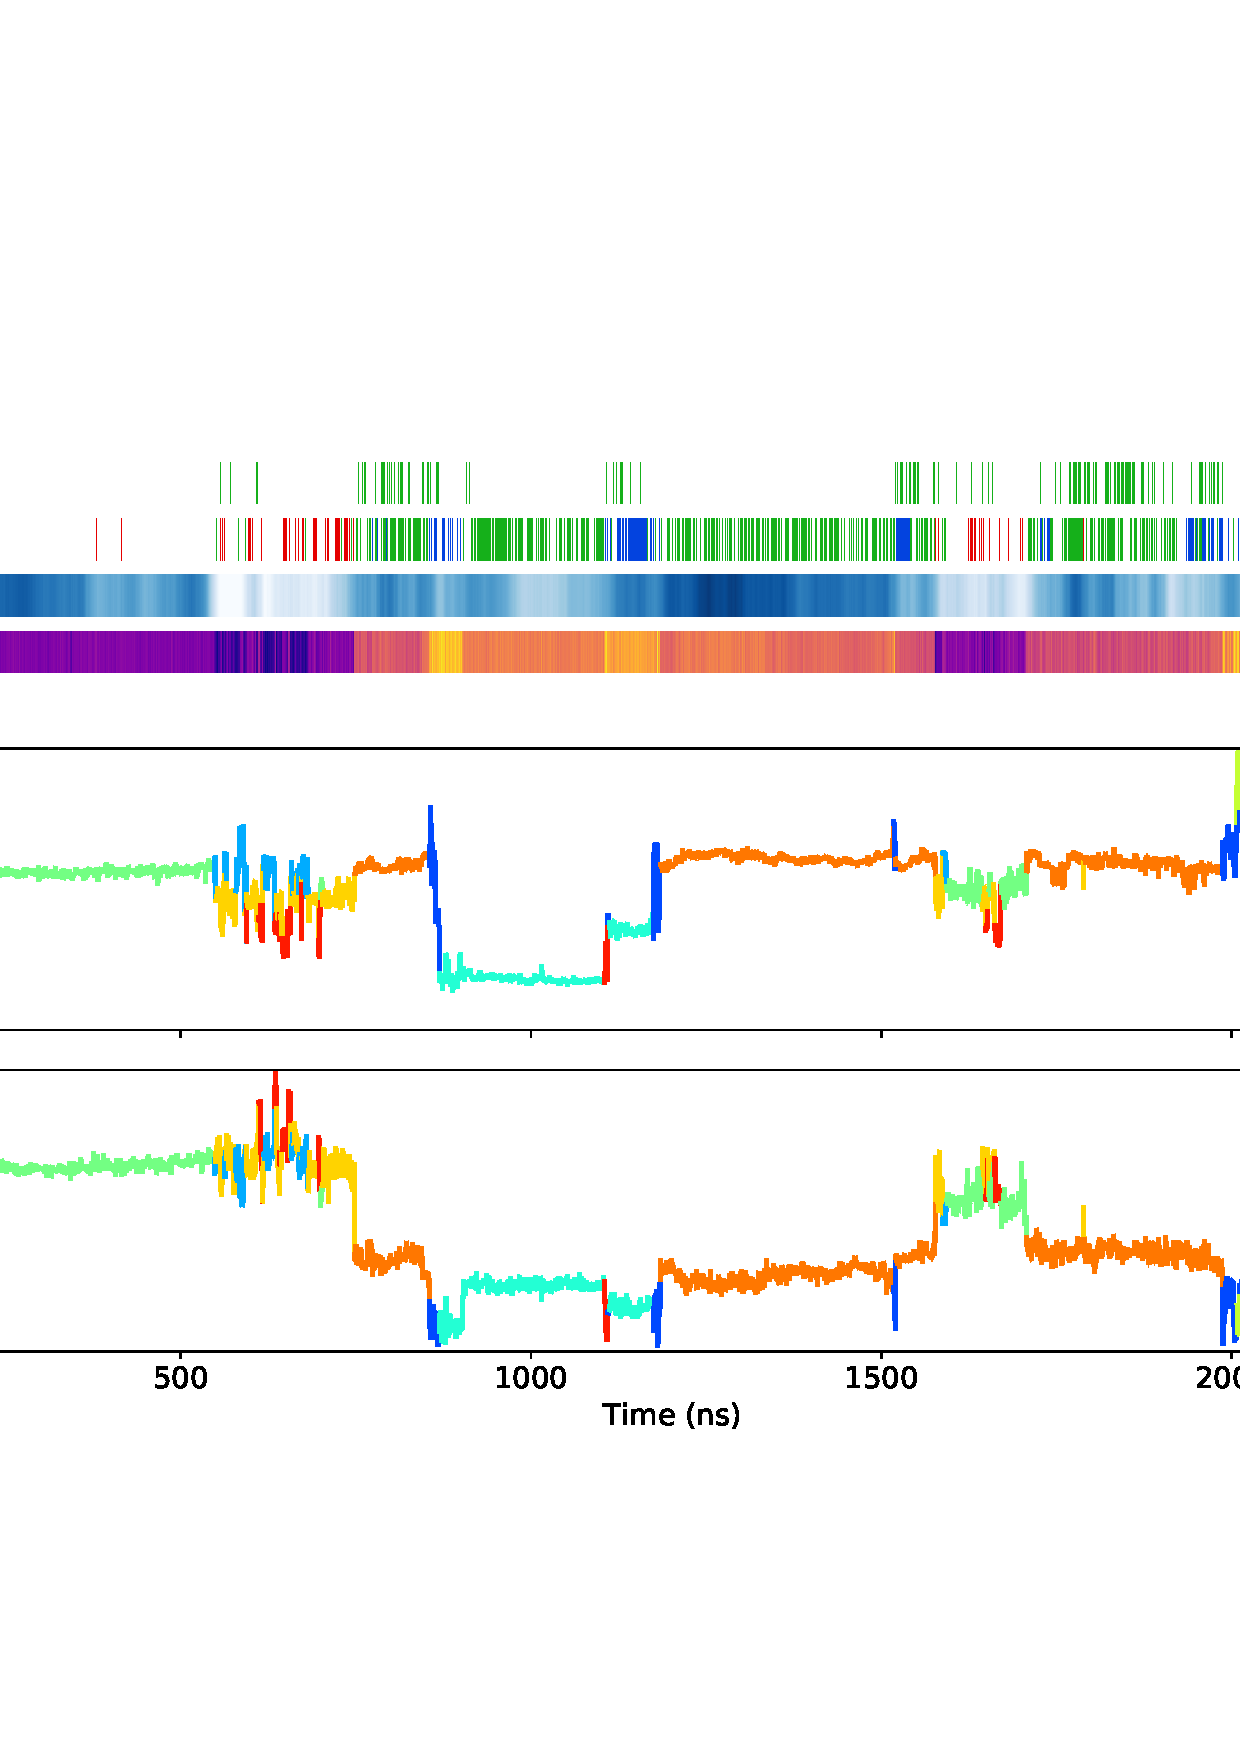
\includegraphics[width=\textwidth]{mechanism_map.png}
  \caption{}
  \end{subfigure}
  \begin{subfigure}{0.24\textwidth}
  \includegraphics[width=\textwidth]{monomer_oxygens.png}
  \caption{}
  \end{subfigure}
  %MRS: a lot of this caption test is duplicated from the main text. I would suggest reducing the duplication.
  %BJC: you think better to have more detail in text or in caption?
  %MRS2: at a certain point, it should be in the text.  In the caption, I would just state what the point of the plot is, 
  % and define the colors/data/etc.  But full explanation would be better in the text. Captions should be scannable quickly,
  % based on how people process papers, and this should be significantly shorter for readability. 
 \caption{(a) We can learn a significant amount of detail about solute motion by viewing 
  solute trajectories color-coded according to their clustered dynamical behavior alongside
  plots of the dominant molecular interactions and descriptions of the membrane's local 
  environment. In the plot above, we show the radial and axial coordinates of a single
  methanol molecule over the course of the equilibrated portion of its MD simulation.
  Disjoint segments of the same color imply the solute behaves similarly at different 
  points of the trajectory because their VAR parameters place them in the same cluster. 
  There are eight distinct dynamical modes exhibited by this trajectory. In order
  of their first appearance, they are colored dark yellow, red, light blue, light green,
  orange, blue, teal and lime green. On the top of the plot are bars which represent different
  physical interactions and the membrane's local environment as a function of time. The top 
  bar is colored green at time points where solutes are associated with sodium. Methanol 
  associates with sodium ions relatively infrequently. The next bar down is colored when hydrogen
  bonds exist. The colors match the enlarged oxygen atoms highlighted in (b). Blue slivers
  correspond to hydrogen bonds donated to the monomer's carboxylate head group. Green slivers
  correspond to  hydrogen bonds donated to the ether linkages between the head groups
  and tails. Red slivers correspond to hydrogen bonds donated to the oxygens on the ends
  of the monomer tails. Methanol exhibits significant hydrogen bonding with all parts of
  the monomer. Which part of the monomer methanol hydrogen bonds to is heavily correlated
  to the solute's $r$ coordinate. Finally, the bar with the blue gradient represents the local 
  membrane density based on the solute's ($r$, $z$) coordinate. Darker shades of blue
  correspond to higher membrane densities. The density appears to be higher when methanol
  motion is restricted (e.g. from 75 to 550 ns). It is relatively low in areas where methanol's
  position fluctuates significantly (e.g. from 550 to 700 ns). 
  }\label{fig:mechanism_map}
  \end{figure}

  %MRS2: suggest subsubcaptions/italics at the start of parentheses to make it easier for a reader to see the structure.
  %MRS2: like \textit{hydrogen bonding patterns}: etc.

  One can gain useful chemical intuition just by studying plots like
  Figure~\ref{fig:mechanism_map}. It is clear that, for methanol, association 
  with sodium is a much rarer interaction than hydrogen bonding with the 
  LLC monomers. Methanol hydrogen bonds to all regions of the monomers dependent
  on its radial position. Its fluctuations tend to be smallest when hydrogen bonded
  or in areas of high local number density. For example, from approximately 75 to 
  525 ns, methanol appears to be trapped in a high density region of the tails.
  In the time that follows, it enters a region of relatively low density where 
  fluctuations are quite large. During this time period, there is intermittent, 
  short-lived hydrogen bonding with the oxygen atoms at the tail ends, as suggested
  by the frequent state changes during that time period and red slivers in the bar
  above. Significant hops in the $z$ direction appear to be described by the dark blue
  state. After entering the dark blue state ca. 850 ns, methanol appears to jump
  significantly in the $z$ direction from a hydrogen bonded state with the ether 
  linkages to a hydrogen bonded state with a head group in a monomer below it.

  %MRS2: not entirely clear about the purpose of this paragraph? Seems to be just saying it's possible to learn more?
  %MRS2: should clarify.
  It is clear that there is a wealth of information in these plots, but they don't give
  the complete picture needed in order to formulate LLC membrane design principles. One
  can analyze each segment sequentially and form a clear picture of this instance of 
  methanol's behavior without the need to visualize the trajectory with software like VMD.~\cite{humphrey_vmd:_1996}
  However, it is still possible to gain a more general understanding of methanol's average
  behavior.
  
  % BJC2: the numbers and choices of states in this paragraph will change, but I think we
  % can still use this framework to study mechanisms.
  We may learn the most by studying the dynamical modes common to the majority of 
  the solute trajectories. Using the IHMM, we identified 33 total dynamical modes 
  exhibited by methanol. Of those, only six states appear in a third (8 out of 24) 
  or more methanol trajectories, and three of them appear in over 50 \% of the 
  methanol trajectories. 12 of the detected states are shared by two or less 
  methanol trajectories. In Figure~\ref{fig:common_states_MET_lines}, we plot 
  representative dynamics of each of the six states which we determined to be prevalent.
  We also chose to study a seventh state, which only appears in three out of
  24 trajectories, because methanol experiences very long periods of entrapment
  while in this state. Long trapping events, even if they are relatively rare, will
  have a significant influence on solute flux. No trajectory contains all seven states.
  However, the trajectory in Figure~\ref{fig:mechanism_map} exhibits all modes except
  states 6 and 7. The states in Figure~\ref{fig:common_states_MET} are colored to match
  states that also appear in Figure~\ref{fig:mechanism_map}.
  
  %BJC2: Again, this will change, but will follow the same general flow
  We can begin to dissect the dynamics of each state by studying their parameters.
  States 1, 3 and 5 have radial means near 1 nm or less (see y axis of $r$ direction 
  plot in Figure~\ref{fig:common_states_MET_lines}), which suggest that they occur
  close to the pore centers. States 2, 4, 6 and 7 occur well within the tail region
  of the membrane. States 1 and 2 have higher covariances in both the axial and radial
  directions compared to all other states. Covariance in each dimension appears to have
  a strong correlation. States 3 and 5 (in the pore region) as well as states 4, 6 and
  7 (in the tail region) are primarily distinguished based on their autoregressive 
  coefficients, A. Higher values of A generally lead to more wandering about the state
  mean. One could argue that the parameters of states 3--7 are actually very close which
  suggests that solutes might behave alike in morphologically distinct regions of the 
  membrane.

  Despite some similarity in their VAR parameters, the length of time spent in states 
  3--7 appears to be dependent on the solute's radial location. Based on the 
  self-transition probabilities, we estimated the average time spent by each solute in
  each state (Figure~\ref{fig:dwell_times_MET}). States 3, 5 and 7 have long dwell times
  relative to the rest because they have high self-transition probabilities. Somewhat 
  surprisingly, both states 3 and 5 correspond to solutes located close to a pore center,
  where one might expect solute motion to be less restricted. Although solutes in states
  4 and 6 are in the viscous tail region, their dwell times are only intermediate. This
  could be due to inhomogeneity in the tail region which causes transitions between many
  different trapped states but with little net effect on solute MSD. However, there are
  instances of states within the tail region with dwell times that exceed 100--200 ns,
  as shown by our inclusion of state 7. There are no other states with dwell times longer
  than state 5 in the pore region.
  
  States 1 and 2 exhibit the shortest dwell times of the states studied. This is 
  consistent with the trajectory in Figure~\ref{fig:mechanism_map}. State 2 is the 
  shortest lived state, appearing to bridge other tail region states. State 1 
  appears to represent a significant hopping state. It has a high covariance and
  occurs near the pore center, where there is less obstruction to solute motion.
  It's dwell time of ca.~8 ns, suggests that solutes stay in this highly mobile 
  state for long enough for their positions to displace significantly.
  
  \begin{figure}
  \centering
  \begin{subfigure}{0.6\textwidth}
  \includegraphics[width=\textwidth]{common_states_MET.pdf}
  \caption{}\label{fig:common_states_MET_lines}
  \end{subfigure}
  \begin{subfigure}{0.35\textwidth}
  \includegraphics[width=\textwidth]{A_sigma_scatter_MET.pdf}
  \caption{}\label{fig:A_sigma_scatter_MET}
  \includegraphics[width=\textwidth]{dwell_times_MET.pdf}  % No errorbars because these are expected values
  \caption{}\label{fig:dwell_times_MET}
  \end{subfigure}
  %MRS: a lot of text here in the caption - think about reducing duplication with the text, and moving some to the text.
  %BJC2: will rework once final plots are made.
  \caption{We can learn the most about methanol's behavior by studying the dynamics
  of the states common to many of the methanol trajectories. In (a), we show representative
  dynamics of six states that are common to more than one third of the solute trajectories. 
  The $y$-axis labels of the $r$ coordinate plot specify the radial mean of each clustered 
  state. The percentage of trajectories in which the states appear are labeled to the right of
  the $r$ plots. States 1--5 appear in the trajectory shown in Figure~\ref{fig:mechanism_map}
  and are colored to match for easy visual comparison. All time series have a mean of zero and are
  shifted to put the mean in line with the $y$-axis labels for the purpose of visualizing them. 
  (b) We can begin to understand the solute behaviors demonstrated in (a) by understanding their VAR 
  parameters. States 1 and 2 have higher covariances in both the axial and radial directions compared
  to all other states. This should lead to significant solute displacement. Covariance in each dimension
  appears to have a strong correlation. 
  %MRS2: correlation with what?
  States 3--6 all have relatively low covariances, which may
  be characteristic of trapped states. They are primarily distinguished based on the magnitude of their 
  autoregressive coefficients, A, and radial means. Higher values of A imply motion which wanders 
  more about the mean. States 1, 3 and 5 have radial means near 1 nm or less, which suggest that they
  occur close to the pore centers. States 2, 4 and 6 occur well within the tail region of the membrane.
  (c) Using the transition probabilities ($p$), we estimated the average time spent within each 
  of the states using 1000 simulations of a Bernoulli process where we continued to draw until transitioning
  out of the state with probability $1 - p$. Of the prevalent states, states 1 and 
  2 exhibit the shortest dwell times alongside their high covariances. States 5 and 7 have the longest dwell times in the pore and tail regions respectively.
  }\label{fig:common_states_MET}
  \end{figure}
  
  Most of what we have learned thus far has been based on the parameters of our
  model with some qualitative validation using a single methanol trajectory. While 
  we may be able to further corroborate our arguments by analyzing more
  individual trajectories, it is more useful to correlate the state behavior with
  solute-membrane interactions.

  %BJC2: A lot of the following will probably be reworked with different clustering scheme
  The types of hydrogen bonding undergone by solutes is dependent on radial
  location (see Figure~\ref{fig:hbond_pichart}). States with radial means near 1 nm
  or less (states 1, 3 and 5) typically hydrogen bond with the monomer carboxylate
  groups and ether linkages. States with radial means greater than 1 nm (states 2,
  4, 6 and 7) tend to hydrogen bond with the monomer tails. 
  %MRS: tweak
  %In the past we've 
  Our previous work has
  shown that there is a gradual transition from the hydrophilic to hydrophobic region in
  these membranes, meaning the monomer location is not tightly bound in $r$. 
  %MRS: above logic is not clear?
  Therefore, there are instances of hydrogen bond interactions that one might consider 
  uncharacteristic based on the state's radial mean.
  %MRS: what is implication of ``uncharacteristicness''? 

  States which exhibit longer dwell times have longer hydrogen bond lifetimes (see
  Figure~\ref{fig:hbond_pichart}). States 3--7 have significantly longer hydrogen 
  bond lifetimes than states 1 and 2. It makes physical and mathematical sense that
  states 1 and 2 should not stay trapped by hydrogen bonding for long periods because
  they typically take large hops as communicated by their large covariances.
  In the tail states, hydrogen bond lifetimes appear to increase with their dwell 
  times. However, in the pores, the same linear relationship does not hold.
  For example, state 5 has the lowest hydrogen bond lifetime of states 3--7
  despite having the second longest dwell times. 
  
  The local density experienced by solutes may have an impact on the length of solute 
  entrapment. On average, solutes in state 5 are surrounded by a relatively high density
  of particles. Based on its radial location and preference towards hydrogen bonding
  with the ether linkages (see Figure~\ref{fig:hbond_pi_charts}), it is reasonable to
  assume that while in state 5, methanol spends most of its time just outside the 
  pore region, sandwiched between the monomer head groups. Although state 5 hydrogen
  bonds break more frequently than one might expect for a state with long dwell times,
  it is possible that the solute's dense surroundings prevent it from wandering off 
  before the hydrogen bonding interaction can be recovered. This may explain the 
  behavior of the methanol in state 5 of the trajectory in Figure~\ref{fig:mechanism_map}
  where the solute's center of mass appears to move more freely about its mean than 
  other trapped states. The data suggests that methanol molecules in state 3 lie closer
  to the pore center than state 5 because they tend to hydrogen bond most frequently 
  with the carboxylate groups. Methanol molecules which experience state 3 are subject 
  to a lower density local environment and rely more heavily on hydrogen bonding interactions, 
  evidenced by their longer lifetimes, to stay trapped.
  
  States describing behavior in the tail region show a direct relationship between 
  hydrogen bond lifetimes and local density. Methanol molecules which experience state 2 
  spend their time in a low density region of the tails where they can easily break free
  of hydrogen bonds. Conversely, methanol molecules trapped in state 7 are in the densest 
  region of all states studied. It is likely difficult for methanol to escape these high 
  density regions and its position is further stabilized via hydrogen bonding.
  
  %BJC4: I didn't put sodium ion association in this figure because it's infrequent. 
  %BJC4: If I compare to acetic acid or urea, I could add it back. I was thinking of splitting
  % the pi chart in half with slices corresponding to hbonds on one side and association on the other
  \begin{figure}
  \centering
  \begin{subfigure}{0.54\textwidth}
  \includegraphics[width=\textwidth]{hbond_pi_charts.pdf}
  \caption{}\label{fig:hbond_pi_charts}
  \end{subfigure}
  \begin{subfigure}{0.45\textwidth}
  \includegraphics[width=\textwidth]{hbond_lifetimes_density_MET.pdf}
  \caption{}\label{fig:hbond_lifetimes_density_MET}
  \end{subfigure}
  %MRS: legend doesn't show stripes.
  \caption{(a) Methanol hydrogen bonds in different segments of the LLC monomer
  dependent on the state. States with mean radial locations in the pore region tend to
  hydrogen bond with the head groups and ether linkages. States with mean radial
  locations in the tails tend to hydrogen bond with the tail oxygen atoms.
  (b) Hydrogen bond lifetimes and the local density experienced by methanol
  molecules can help us to understand dynamical states in terms of membrane 
  interactions. The bars are colored according to match the states in Figures~\ref{fig:mechanism_map}
  and~\ref{fig:common_states_MET}. States 1 and 2, which have large covariances, also have short
  hydrogen bond lifetimes and exist in relatively low density regions. The
  hydrogen bond lifetimes of methanol in states with radial means in the tail
  region tend to increase with local density and mean dwell times. 
  %MRS7: not clear from graphic which ones are in the pore.
  %MRS7: is there any legend for the color for b? If same as above figure, indicate. Don't REALLY need color since they bars are already labeled, so it's 2 sources of duplicate information.
  %BJC7: The state numbers are all you need to compare to the previous figure BUT the color make it easier 
  %plot of the methanol trajectory where states aren't labeled.
  %MRS7: cross-hatching doesn't appear in the legend? Not sure which is which (I assume hatched is number density because closer to that axis).
  %BJC7: Is it because the hatches aren't dense enough? I see them in the legend
  This monotonic
  relationship does not exist for states in the pore region. The high 
  local density experienced by state 5 methanol molecules may explain why 
  hydrogen bond lifetimes are short but dwell times are high. State 5 methanol's
  preference towards hydrogen bonds with ether linkages suggests that the solute
  sits between LLC monomer head group which prevent it from wandering to far
  before recovering its previous hydrogen bond.
  }\label{fig:hbond_pichart}
  \end{figure}
  
  \subsubsection*{Comparison of Solute Behavior}
  %BJC2: Again, most of this section will get a facelift, but will try to follow same flow 
  We applied similar analysis to the other three solutes in this study: urea, acetic acid
  and ethylene glycol. Not only can we use the model to study the dynamics of each 
  solute individually, but we can compare their behavior in order to improve our
  understanding of more subtle mechanistic details.
  
  The size and chemical functionality of the solutes dictates the interactions which
  influence solute transport. In Figure~\ref{fig:hbonds_assoc_summary}, we show that
  the solutes donate hydrogen bonds and associate with sodium ions to varying degrees.
  We also show the solute MSDs after a 1000 ns time lag. It is not immediately obvious
  why the MSDs follow this trend. 
  %MRS2: be more precise what ``this trend'' is.
  The states identified by the IHMM shed
  some light on the reasoning.
  
  \begin{figure}
  \centering
  \begin{subfigure}{0.45\textwidth}
  \includegraphics[width=\textwidth]{hbonds_assoc_summary.pdf}
  \caption{}\label{fig:hbonds_assoc_summary}
  \end{subfigure}
  \begin{subfigure}{0.45\textwidth}
  \includegraphics[width=\textwidth]{rdf_summary.pdf}
  \caption{}\label{fig:rdf_summary}
  \end{subfigure}
  \begin{subfigure}{0.45\textwidth}
  \includegraphics[width=\textwidth]{dwell_time_summary.pdf}
  \caption{}\label{fig:dwell_time_summary}
  \end{subfigure}
  \begin{subfigure}{0.45\textwidth}
  \includegraphics[width=\textwidth]{cov_summary.pdf}
  \caption{}\label{fig:cov_summary}
  \end{subfigure}
  %MRS7: is c) methanol?  I thought it wasn't associating with Na+ much.
  %BJC7: looks about 5 %, certainly less than the other. I could add
  % some discussion of this to previous section.
  %MRS: methanol yellow is hard to see in (b). Maybe add outlines to histogram?  I guess they are, increase alpha or something for yello?
  %MRS: check consistency of capitalization in legend in (c) 
  \caption{(a) Solutes hydrogen bond and associate with sodium ions
  to different degrees. Sometimes, they participate in both interactions at
  once. The frequency at which solutes interact via either mechanism does
  not appear to be linearly related to the solute's mean squared displacement
  after a 1000 ns time lag. (b) We histogrammed the means of the clusters weighted
  by the number of fluctuation within that cluster. Most solutes spend the majority of
  their time close to the pore center. Only methanol has a significant peak
  beyond 1.5 nm from the pore center. (c) The trend in the maximum dwell time
  among prevalent states for each solute is inversely related to the
  solute's MSD. In some cases, non-prevalent states show very long dwell times,
  which may have a significant impact on solute MSD. (d) All solutes tend to
  take larger hops in the $z$ direction when they are in the pore versus in 
  the tails. All solutes except urea make slightly larger radial hops while 
  in the tails.
  %BJC6: I made this plot out of curiosity, not sure if I'll use it yet.
  }\label{fig:summaries}
  \end{figure}
  
  Hydrogen bonding and sodium ion association interactions are far more 
  common when solutes stay near the pore centers. In Figure~\ref{fig:rdf_summary},
  we plot the distribution of the radial means of each cluster weighted by 
  the time spent in that cluster. All solutes except methanol spend the 
  majority of their time near the pore centers (roughly defined as within 
  1.5 nm). As we showed earlier, methanol spends a significant portion of its
  time trapped in the dense tails.
  
  % BJC: we can probably use this to create a new definition of the pore and tail region.
  % and perhaps focus on transitions between them.
  Solute size likely has a large effect on their preferred radial location within
  the pores. The histograms in Figure~\ref{fig:rdf_summary} have a clear vacancy 
  between what one might consider the pore and tail region, most evident in methanol's 
  distribution of radial positions. The area between the head groups and the distal
  regions of the tails is dense and hydrophobic which creates a considerable energy 
  barrier to be overcome in order to transition to that region.
  %BJC: I wonder if there is a state which corresponds to the jump from pore to tail region. Might be hard to pick up.
  Methanol is the smallest solute in this study and therefore appears to 
  have the easiest time crossing into the tails.

  Despite their close proximity to the low density aqueous pore region, acetic
  acid, ethylene glycol and urea exhibit a range of trapping behavior.
  It is clear that the number of polar interactions is not directly
  related to solute MSD. Acetic acid participates in a similar number of 
  interactions relative to urea and ethylene glycol, but its MSD is considerably
  lower. For the purpose of this analysis, as in the previous section, we 
  defined states that appear in more than one third of the trajectories to
  be prevalent states. In Figure~\ref{fig:dwell_time_summary}, we plot the\
  longest dwell times exhibited by each solute among the prevalent states as 
  well as out of all the states. The state which exhibits the longest dwell
  times among all acetic acid states appears in 9 different trajectories, 
  making it a prevalent state, and occurs 0.9 nm from the pore center.
  Although urea possesses the state with the longest dwell time among the
  solutes studied, it occurs in the tail region with prevalent states having 
  much shorter dwell times. Ethylene glycol appears to be the least subject to
  trapping.

%  The combination of a carbonyl group, which binds strongly to sodium, and a 
%  hydroxyl group, which can form strong hydrogen bonds, makes acetic acid
%  particularly prone to trapping.
%  BJC6: more complicated than this. I will revisit.
  
  \section{Conclusion}
  
  We have shown that the IHMM can be used to automatically parameterize solute 
  time series with an unknown number of latent dynamical modes. Initially, we applied
  the algorithm to each trajectory independently. For each solute studied, this resulted
  in over 300 distinct states. By clustering the parameter sets we were able to reduce 
  the state space to 10\% of its original size by grouping states with similar VAR
  parameters.
  
  We coupled analysis of the clustered parameter sets with measurements of membrane 
  properties and solute-membrane interactions in order to gain a detailed understanding
  of the diverse sets behavior exhibited by solutes in these membranes. We showed how
  solute motion is influenced by hydrogen bonding, sodium ion association and local
  membrane density. These interactions have a direct impact on the size and
  correlation of sequential solute steps.
  
  % BJC6: I'll weaken this for the thesis, but this is what I hope to say in the 
  % final paper.
  Finally, we show how one can generate stochastic realizations of our model that
  can qualitatively and quantitatively reproduce the behavior of MD solute 
  trajectories. The realizations show the hopping and trapping behavior that is
  characteristic of polar solutes in this system. We can also use them to reproduce
  the solute MSDs measured from the MD trajectories. The low computational expense 
  of generating these stochastic trajectories allows one to project solute behavior
  on much longer timescales and thus predict experimentally-relevant macroscopic 
  transport properties like solute flux and selectivity.
  
  We showcase this modeling approach by example, but it is important to
  recognize the generality of this analysis, especially in the context of molecular
  simulations. Vector autogregressive models can describe a diverse set of behavior
  and so the IHMM may be suited to study many types motion, including those not 
  characterized by hopping and trapping. The IHMM is a powerful approach for 
  understanding particle motion as well as for generating inexpensive models
  which can give macroscopic insight.
  
  \section*{Supporting Information}

  Detailed explanations and expansions upon the results and procedures mentioned in
  the main text are described in the Supporting Information. 
  %This information is
  %available free of charge via the Internet at http://pubs.acs.org.

  \section*{Acknowledgments}

  This work was supported in part by the ACS Petroleum Research Fund
  grant \#59814-ND7 and the Graduate Assistance in Areas of National Need (GAANN) 
  fellowship which is funded by the U.S. Department of Education. 
  Molecular simulations were performed using the Extreme Science and
  Engineering Discovery Environment (XSEDE), which is supported by National
  Science Foundation grant number ACI-1548562. Specifically, it used the Bridges
  system, which is supported by NSF award number ACI-1445606, at the Pittsburgh
  Supercomputing Center (PSC). This work also utilized the RMACC Summit supercomputer,
  which is supported by the National Science Foundation (awards ACI-1532235 and
  ACI-1532236), the University of Colorado Boulder, and Colorado State
  University. The Summit supercomputer is a joint effort of the University of
  Colorado Boulder and Colorado State University.

  \clearpage

  \bibliographystyle{ieeetr}
  \bibliography{hdphmm}

  %\newpage

  %\section*{TOC Graphic}

\end{document}

% LocalWords:  BJC micropollutants Desalination permeability nanofiltration LLC
% LocalWords:  Amphiphilic nanostructures Lyotropic amphiphilic lyotropic MSDDM
% LocalWords:  solutes selectivities solute nanoscopic timescales MSDs MSD HMMs
% LocalWords:  nonparameteric Parrinello Rahman barostat rescale transitioning
% LocalWords:  al's HMM Dirichlet HDP DP Wishart TODO SI al MATLAB teh gael pdf
% LocalWords:  nonparametric bayesian solute's reparameterized intracluster ca
% LocalWords:  delocalize Luzar Chandler histogrammed interpolator methanol's
% LocalWords:  nanostructure carboxylate VMD nonidealities hbonds outlier GAANN
% LocalWords:  autogregressive PRF ACS XSEDE ACI
